\subsection{Problema a resolver}
El siguiente ejercicio consiste en hallar una manera de implementar un sistema proporcionado respetando una cota determinada de orden de complejidad. El problema se sitúa en un centro de distribución de correo que recibe paquetes todos los días cuyo destino final es la sede central de la empresa. Para el transporte de los mismos, éstos son cargados a camiones de igual capacidad. El encargado de logística, Pascual, tiene un sistema que utiliza desde hace años para agilizar la carga de los camiones asegurando el uso de una baja cantidad de los mismos para el envío de paquetes al final del día. Dicho sistema consiste en agarrar los paquetes y ubicarlos en algún camión que ya tenga paquetes dentro, eligiendo entre éstos el que menos peso esté cargando hasta ese momento. Si el peso del paquete permite que éste sea cargado en ese camión, se lo ubica allí, sino, se lo incluye en un nuevo camión.\newline
El problema a resolver se basa en escribir un algoritmo que tome los pesos de los paquetes que hay que acomodar e indique cuántos camiones se van a utilizar y cuánto peso se cargará en cada uno de ellos al final del día considerando el sistema de Pascual. Para esto, se respeta el orden de llegada de los paquetes a medida que ingresan. \newline
Las consideraciones a tener en cuenta son que los camiones tienen la misma capacidad de carga, la cantidad disponible de los mismos alcanza para transportar todos los paquetes y que el peso de un paquete no supera la capacidad de carga de un camión. Del mismo modo, el tamaño de los paquetes no es tenido en cuenta.\newline
\newline
\textbf {{Formatos de entrada y salida:}}\newline
\newline
La entrada contiene varias instancias del problema. Cada instancia consta de una línea con el siguiente formato:

$$L\ n\ p_{1}\ p_{2}\ ...\ p_{n}$$


donde \textbf{$L$} es el límite de carga de los camiones, \textbf{$n$} es la cantidad de paquetes a acomodar y \textbf{$p_{1}$, ..., $p_{n}$} son los pesos de cada paquete en el orden en el que deben ser almacenados.\newline

La salida debe contener una línea por cada instancia de entrada, con el siguiente formato:

$$k\ c_{1}\ c_{2}\ ...\ c_{n}$$


donde \textbf{$k$} es la cantidad de camiones utilizados y \textbf{$c_{1}$, ..., $c_{k}$} es el peso que se cargó en cada uno de los \textbf{$k$} camiones al final del día.\newline

En lo que sigue, presentaremos dos ejemplos sobre el sistema impulsado por Pascual:
\begin{itemize}
\item \large{\textbf{Ejemplo 1:}}\newline

\textbf{Formato de entrada:}
$$100\ \ 5\ \ 20\ \ 40\ \ 80\ \ 15\ \ 100$$

\begin{figure}[H] %[h] Aqui [b] para button [t] para top
\begin{center}
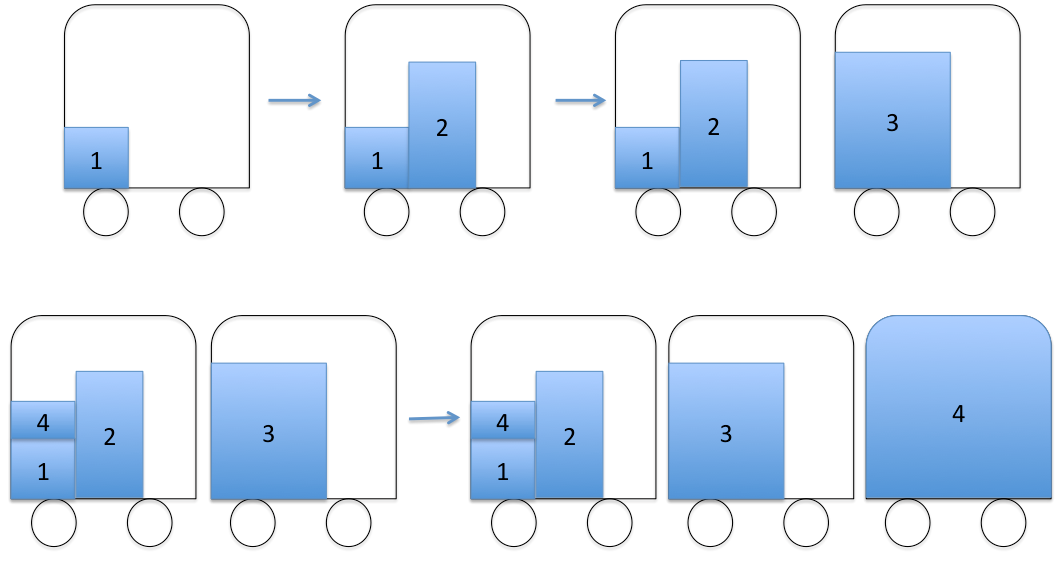
\includegraphics[width=320pt]{../imgs/ejemplo1.jpg}
\end{center}
\end{figure}

\textbf{Formato de salida:}
$$3\ \ 75\ \ 80\ \ 100$$

\item \large{\textbf{Ejemplo 2:}}\newline

\textbf{Formato de entrada:} 
$$150\ \ 3\ \ 80\ \ 75\ \ 82$$

\begin{figure}[H] %[h] Aqui [b] para button [t] para top
\begin{center}
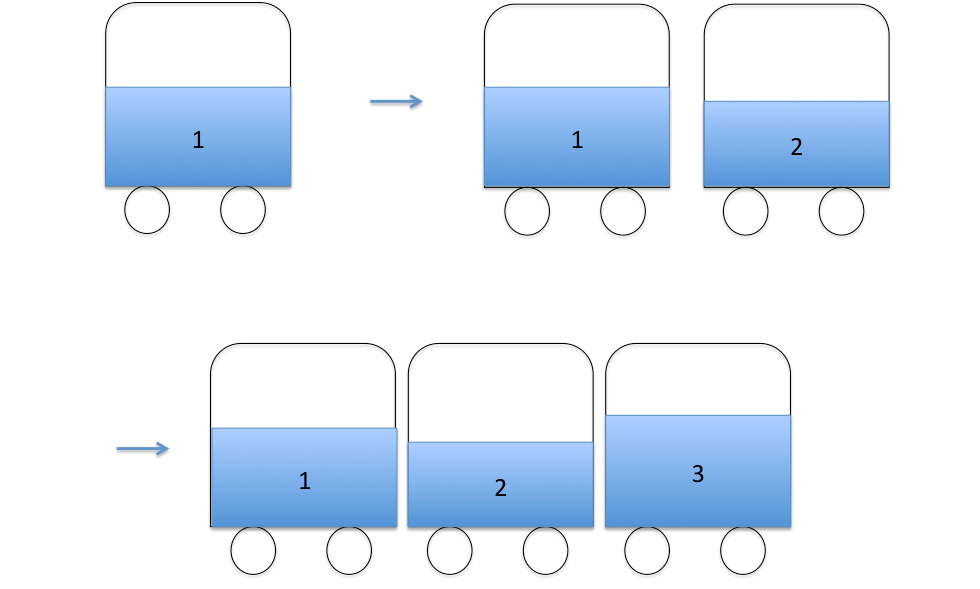
\includegraphics[width=300pt]{../imgs/ejemplo2.jpg}
\end{center}
\end{figure}

\textbf{Formato de salida:}
$$3\ \ 80\ \ 75\ \ 82$$


\end{itemize}
\subsection{Resolución coloquial}


\subsection{Demostración de correctitud}

\subsection{Complejidad del algoritmo}
Tal como requerido, la complejidad temporal del algoritmo debe ser estrictamente menor a $\mathcal{O}(n^2)$.


\subsection{Código fuente}



\subsection{Instancias posibles}



\subsection{Testing}
